%!TEX root = ../main.tex
\chapter{Introdução}

\section{Motivação}

A nossa audição é um dos nossos sentidos mais importantes. É ela que nos permite identificar sinais e padrões no nosso mundo. Desde os tempo antigos, utilizamos a nossa audição para identificar situações de ameaças iminentes, como o rugido um predador prestes a atacar ou a buzina de um carro em alta velocidade. É também através dela que desenvolvemos o nossos métodos de comunicação.

As indústrias de entrenimento (filmes, músicas, games e etc) utilizam o som para criar um ambiente imersivo para o usuário, criando experiências mais realistas e divertidas. Uma das ténicas mais utilizadas por essa indústrica é chamada de Foley. Nessa técnica, o artista de Foley utiliza elementos e objetos do mundo real para tentar sintezar as amostras de áudio de uma cena. O artista pode, por exemplo, utilizar pedaços de côcos para simular o som do trote de um cavalo \cite{bonebright2012were} ou folhas metálicas para simular o som de trovões (Ver \figref{fig:foley}).

\begin{figure}[ht]
	\centering
	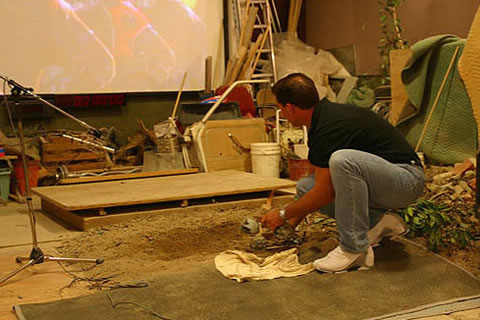
\includegraphics[width=0.6\textwidth]{introduction/foley.jpg}
	\caption[Artista de Foley em um estúdio de produção]{Artista de Foley em um estúdio de produção\footnotemark}\label{fig:foley}
\end{figure}

\footnotetext{Fonte: \url{http://www.t.sonypicturesstudiostours.com/uploads/img/std_content/soundeffects_05.jpg}. Acessado em 3 de Julho de 2016.}

Essa técnica, porém, tem várias limitações. A prática de Foley requer mão-de-obra especializada. Além disso, o tempo de produção escala linearmente com a quantidade de amostras sonoras desejadas. Essa combinação de fatores faz com que o custo da Técnica de Foley seja alto. Em muitos casos também há limitações físicas envolvidas. Seria inviável, por exemplo, usar esse tipo de técnica para sintetizar amostras de áudio geradas por uma estrutura metálica de grandes dimensões ou por uma grande esfera de platina.

Em ambientes dinâmicos, no entanto, as limitações são ainda mais aparentes. O uso de amostras sonoras cria um ambiente acústico repetitivo que não se adapta à realidade do mundo virtual. Esse tipo de técnica não permite que o som dos objetos seja alterado de acordo com o estado da simulação em tempo de execução. O som gerado por um prato ao cair no chão, por exemplo, varia drasticamente de acordo com a posição de contato. Esse tipo de comportamento não pode ser simulado adequadamente com o uso de amostras sonoras.

Para resolver esse tipo de problema, um novo ramo da Computação vem crescendo: o ramo da Computação Acústica. Um dos problemas mais interessantes da área é exatamente o problema da Síntese de Áudio Realístico: Dada a especifição de uma cena (geometria dos objetos, materiais dos objetos) e dados os parâmetros dos materiais presentes, como podemos sintetizar o áudio dessa cena? A solução desse problema resolveria exatamente as dificuldades que temos com as técnicas atuais. Isso nos permitiria criar experiências virtuais mais ricas e fiéis à realidade com apenas uma fração do custo atual de produção. 

\section{Objetivos}

O objetivo desse trabalho é descrever os principais conceitos e também o estado-da-arte da área de Síntese de Aúdio Realístico. Além disso, também queremos desenvolver um método para acelerar a computação da Radiação Acústica em GPU.

\section{Estrutura do Trabalho}

Esse trabalho está estruturado da seguinte maneira: No Capítulo 2 descrevemos os conceitos matemáticos utilizados no estado-da-arte, o que inclui conceitos de Acústica e de Vibrações. No Capítulo 3 descrevemos os trabalhos relacionados, apresentando a evolução da área e discutindo as diferençãs entre métodos Physically-Based e métodos Data-Driven. No Capítulo 4 nós apresentamos o nosso método para calcular a Radiação Acústica em GPU e também os detalhes de implementação. No Capítulo 5 nós descrevemos os experimentos utilizados para avaliar o desempenho do nosso método e também discutimos os resultados obtidos. Finalmente, concluímos esse trabalho no Capítulo 6 apresentando também planos para trabalhos futuros.
